\documentclass{template/openetcs_report}
% Use the option "nocc" if the document is not licensed under Creative Commons
%\documentclass[nocc]{template/openetcs_report}
\usepackage{lipsum,url}
\graphicspath{{./template/}{.}{./images/}}


\begin{document}
\frontmatter
\project{openETCS}

%Please do not change anything above this line
%============================
% The document metadata is defined below

%assign a report number here
\reportnum{OETCS/WP2/D2.2}

%define your workpackage or task here
\wp{openETCS@ITEA Work Package 2: ``Requirements''}

%set a title here
\title{CENELEC EN 50128:2011 Requirements for openETCS}

%set a subtitle here
%\subtitle{CENELEC EN 50128:2011 Requirements for openETC}

%set the date of the report here
\date{June 2013}

%define a list of authors and their affiliation here
\author{Merlin Pokam \and Norbert Sch\"afer}

\affiliation{AEbt Angewandte Eisenbahntechnik GmbH\\
  Adam-Klein-Stra\ss e 26\\
  90429 N\"urnberg\\
  Germany}


% define the coverart
\coverart[width=350pt]{openETCS_EUPL.png}

%define the type of report
\reporttype{Final Report}


\begin{abstract}
This document gathers requirements coming from the CENELEC standards, particularly the CENELEC standard EN 50128:2011, that shall be fulfilled, in order to prove that the deliverables of the openETCS project are fit for theirs intended purposes and respond correctly to safety issues that have been derived from the hazard analysis and risk assessment.
\end{abstract}

%=============================
%Do not change the next three lines
\maketitle

\begin{tabular}{|p{4.4cm}|p{8.7cm}|}
\hline
\multicolumn{2}{|c|}{\textbf{Document information}} \\
\hline
Work Package &  WP2  \\
Deliverable ID or doc. ref. & D2.2\\
\hline
Document title & CENELEC EN 50128:2011 Requirements for openETCS \\
Document version & 2.0.0 \\
Document authors (org.)  & Merlin Pokam (AEbt) \\
\hline
\end{tabular}

\begin{tabular}{|p{4.4cm}|p{8.7cm}|}
\hline
\multicolumn{2}{|c|}{\textbf{Review information}} \\
\hline
Last version reviewed & 1.2.0 \\
\hline
Main reviewers & Jan Welte,  Marielle Petit-Doche, Jonas Helming, Stefan Rieger, Marc Behrens, Cecile Braunstein, Armand Nachef, Bernd Hekele, Cyril Cornu\\
\hline
\end{tabular}

\begin{tabular}{|p{2.2cm}|p{4cm}|p{4cm}|p{2cm}|}
\hline
\multicolumn{4}{|c|}{\textbf{Approbation}} \\
\hline
  &  \textbf{Name} & \textbf{Role} & \textbf{Date}   \\
\hline  
Written by    &  Merlin Pokam & D2.2 Task Leader  & 14/06/13\\
\hline
Approved by &  Gilles Dalmas & WP2 Leader & \\
\hline
\end{tabular}

\begin{tabular}{|p{2.2cm}|p{2cm}|p{3cm}|p{5cm}|}
\hline
\multicolumn{4}{|c|}{\textbf{Document evolution}} \\
\hline
\textbf{Version} &  \textbf{Date} & \textbf{Author(s)} & \textbf{Justification}  \\
\hline  
0.0.0 & 10/02/13 & Merlin Pokam &  Document creation  \\
\hline  
1.0.0 & 20/03/13 & Merlin Pokam &  Updated, version for review  \\
\hline
1.1.0 & 04/04/13 & Merlin Pokam &  The version of the report has been updated from "Preliminary" to "Intermediate" , version for review  \\
\hline
1.2.0 & 08/04/13 & Merlin Pokam &  Updated, version for review  \\
\hline
2.0.0 & 11/06/13 & Merlin Pokam &  Creation of the Final version  \\
\hline
\end{tabular}


\tableofcontents
\listoffiguresandtables
%=============================
% The actual document starts below this line
%=============================



%Start here
%Chapter

\chapter{Abbreviations}

\begin{table} [h]
\begin{tabular}{|p{2cm}|p{12cm}|}
%{
%\footnotesize\sffamily\centering
%  \begin{longtable}{||l|l||}
    \hline\hline
    \bfseries Terms & \bfseries Definition\\
    \hline\hline
%    \endhead
%    \hline\hline
%    \endfoot
    ATC & Automatic Train Control\\
    \hline
    FM & Formal Methods\\
    \hline
    CENELEC & (english) European Committee for Electrotechnical Standardization\\
    \hline
    COTS & Commercial off-the-shelf software, software defined by market-driven need, commercially available   and whose fitness for purpose has been demonstrated by a broad spectrum of commercial users\\
    \hline
    CV & Curriculum Vitae\\
    \hline
    ETCS & European Train Control System\\
    \hline
    ERTMS & European Rail Traffic Management System\\
    \hline
    EUC & Equipment under control\\
    \hline
    FLOSS & free-libre / open source software\\
    \hline
    EN & European Norm\\
    \hline
    ERA & European Railway Agency\\
    \hline
    EVC & European Vital Computer\\
    \hline
    HW & Hardware\\
    \hline
    ISO & International Organization for Standardization\\
    \hline
    OBU & On Board Unit\\
    \hline
    OS & Operating System\\
    \hline
    PCA & Project Co-operation Agreement\\
    \hline
    PO FPP & Project Outline Full Project Proposal\\
    \hline
    RTOS & Real Time Operation Systems\\
    \hline
    SIL & Safety Integrity Level\\
    \hline
    SSIL & Software Safety Integrity Level\\
    \hline
    SRS & System Requirement Specification \\
    \hline
    SRSS & Sub-System Requirement Specificationn \\
    \hline
    STI & Standard Train Interface \\
    \hline
    TSI & Technical Specification for Interoperability\\
    \hline
    UNISIG & UNion Industry of SIGnalling\\
\hline
%\end{longtable}
%}
\end{tabular}
\\
\caption{Abbreviations}
\end{table}


\mainmatter


\chapter{Terms and definitions}
\label{common-terms}

\begin{figure}[h]
  \centering
  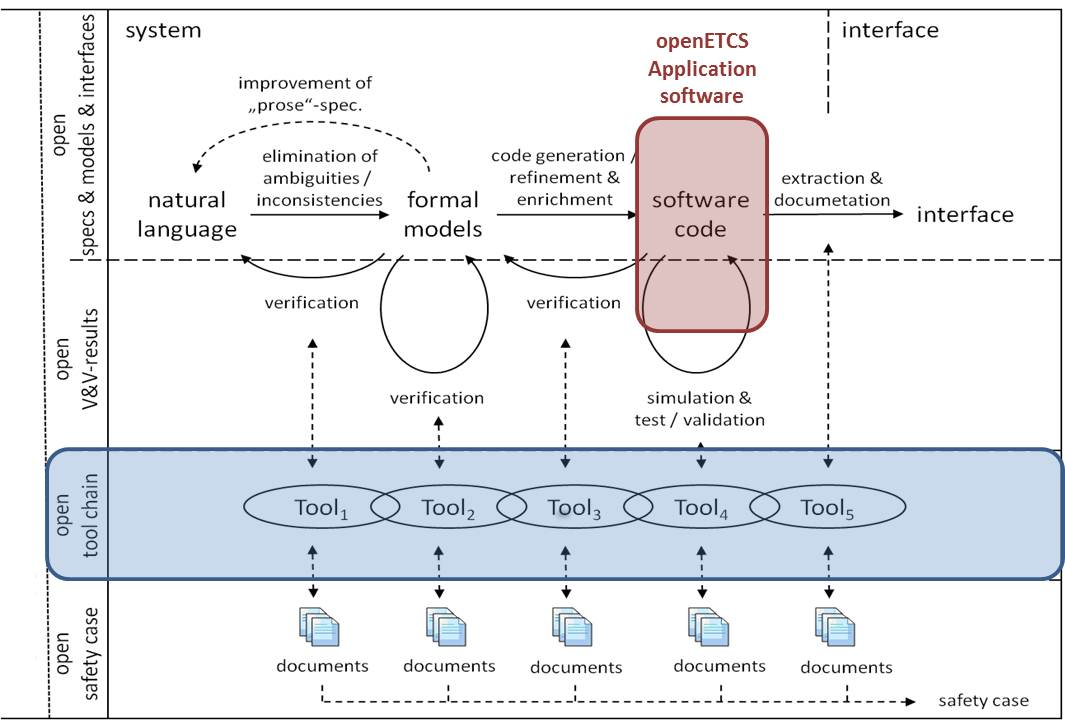
\includegraphics[width=16cm]{openETCS1}
  \caption{openETCS: the holistic approach}
  \label{fig:openETCS1}
\end{figure}

\section{openETCS tools chain}
Set of tools, that covers the entire software development process of the ETCS OBU,
starting from a conventional natural language specification over a formalization of the ETCS OBU system
description for the modeling with verification steps, through to code generation
and automatic generation of documents, see Figure \ref{fig:openETCS1}.\\

\section{openETCS application software}
Software code generated from formal models and not the basis software, see Figure \ref{fig:openETCS1} above.\\


\section{Common terms and definitions}
\begin{table} [h]
\begin{tabular}{|p{2cm}|p{9cm}|p{3cm}|}
\hline
\bfseries Terms & \bfseries Definition & \bfseries Source \\ 
\hline 
\hline
formal specification  & A formal specification is a concise description of the behavior and properties of a system written in a mathematically-based language, specifying what a system is supposed to do as abstractly as possible, thereby eliminating distracting detail and providing a general description resistant to future system modifications. The most formal specifications are written in a language with a well-defined semantics that supports formal deduction and allows the consequences of the specification to be calculated through proof of putative theorems. & \cite{FM-doc}\\ 
\hline
formal proof  & A formal proof is a complete and convincing argument for the validity of a statement about a system description. A proof proceeds in a series of steps, each of which draws conclusions from a set of assumptions. Justification for each step is derived from a small set of rules which state what conclusions can be reasonably drawn from assumptions. Such justification eliminates ambiguity and subjectivity from the argument. Formal proofs may be prepared manually or, preferably, with the assistance of an automated FM tool. & \cite{FM-doc}\\ 
\hline
Open-Source-Software & Source code available to the general public with relaxed or non-existent copyright restrictions & EN 50128:2011 \\ 
\hline
Pre-existing software & All software developed prior to the application currently in question is classed as pre-existing software including: 
\begin{itemize}
\item COTS (commercial off-the-shelf) and open source software,
\item Software previously developed.
\end{itemize} & EN 50128:2011 \\ 
\hline
Open Proofs & An "open Proofs" is software or a system where all of the following are free-libre / open source software (FLOSS): 
\begin{itemize}
\item the entire implementation,
\item automatically-verifiable proof(s) of at least one key property, and,
\item required tools (for use and modification).
\end{itemize} & www.openproofs.org \\ 
\hline
Software & Intellectual creation comprising the programs, procedures, rules, data and any associated documentation pertaining to the operation of a system & EN 50128:2011 \\ 
\hline
Application software & Part of the software of a programmable electronic system that specifies the functions that perform a task related to the EUC rather than the functioning of, and services provided by the programmable device itself & IEC 61508-4:2010 \\ 
\hline
\end{tabular}
%\hline
\\
\caption{Terms and definitions}
\end{table}


\chapter{Introduction and motivation}
In all over Europe there are about 30 different, mostly not compatible signaling and train protection systems in use. For a unified european rail system it is very costly to maintain this diversity of signaling systems and therefore the european commission has set new rules by so called Technical Specifications for Interoperability (TSI, see the latest decision \cite{TSI-doc}) with the goal to implement an unified "European Train Control System (ETCS)", see Figure \ref{fig:openETCS2}.

\begin{figure} [h]
\centering
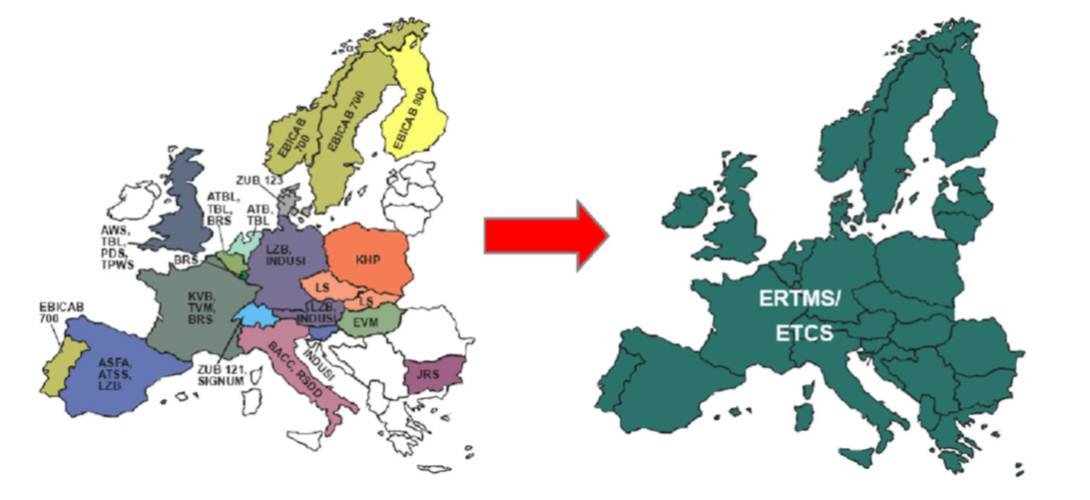
\includegraphics[width=12cm]{openETCS2}
\caption{Substitution of different signaling and ATP systems in the european union by just one unique system: the ETCS}
\label{fig:openETCS2}
\end{figure}

ETCS shall replace national legacy signaling and train control systems and consists of facilities in the infrastructure and in the train: on-board units (OBU). ETCS is a so called cab-signaling system, which means that in principle all commands for the driver are shown on screens inside the driver's cabin, making conventional track-side signals obsolete, resulting in considerable savings for the infrastructure operators. The shift of functionality and safety responsibilities from the infrastructure into the vehicle has caused an increase of complexity for the on-board equipment. In terms of technology, this migration is mostly done by software. While electronic hardware is getting continuously cheaper, the high complexity of the safety critical software has caused significant cost increases for the development, homologation and maintenance of the ETCS.
Despite the fact that several major European suppliers with substantial knowledge in signaling technology have worked on a common System Requirement Specification (SRS, see the latest baseline \cite{SRS-doc} ) for over a decade, the main goal of interoperability has not yet been accomplished. Up to now, not a single ETCS onboard unit has been approved to operate on all existing European ETCS lines. One of the reasons is given by the fact that a plain English specification text "prose" of some complexity cannot be so precise and free of potential divergent interpretation that the resulting software products would behave identical, see Figure \ref{fig:openETCS3}. Therefore the development of ETCS has to be considered as "work in progress", resulting in many software upgrades to be expected in the near and distant future.

\begin{figure}[h]
\centering
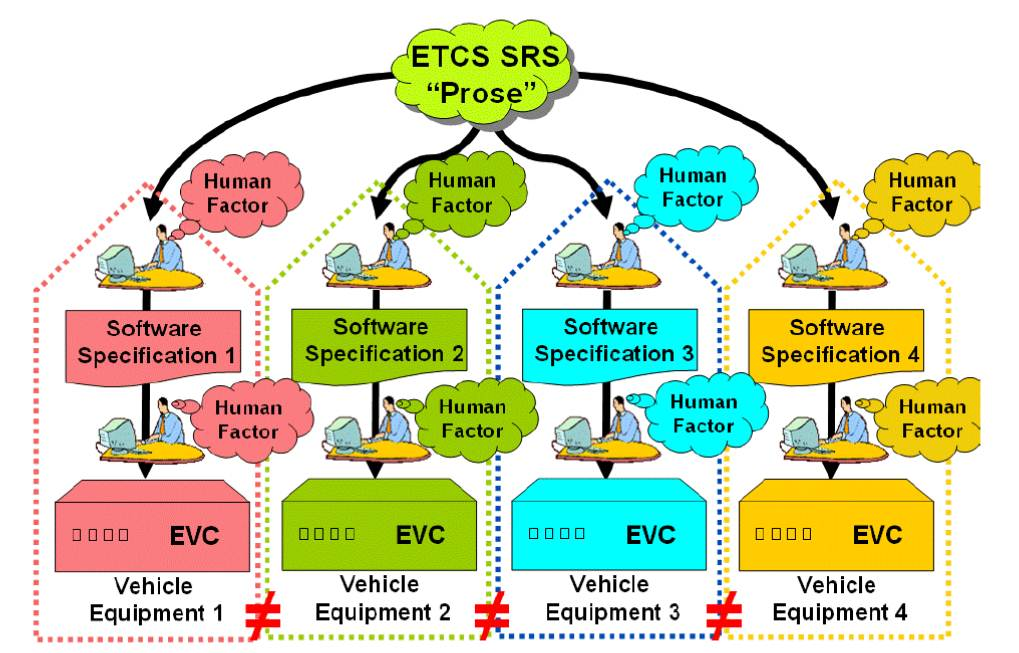
\includegraphics[width=12cm]{openETCS3}
%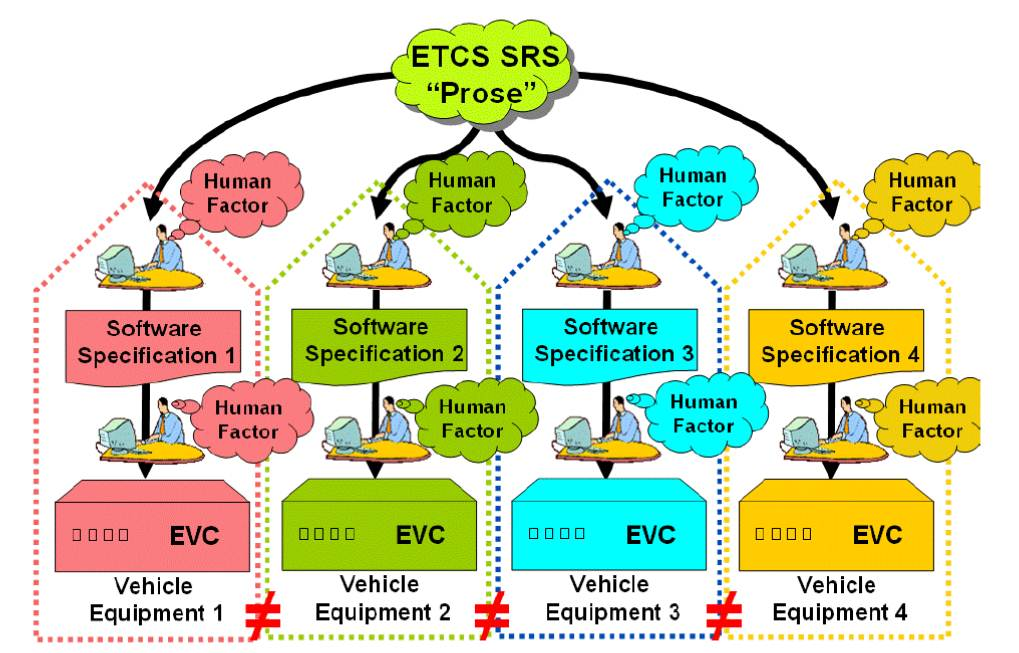
\includegraphics[width=1.0\textwidth, height=240px]{openETCS3}
\caption{Divergent interpretation of a common "informal" ETCS SRS document due to the "human factor".}
\label{fig:openETCS3}
\end{figure}

Almost all products on the market are based on different proprietary software designs, which results in a life-long dependency from the original manufacturers causing high life-cycle costs for vehicle owners. The key element for improving that situation seems to be a greater degree of standardization for: Hardware, software, methods and tools.

An approach following the open source idea, called "openETCS" utilizing concepts from the automotive and
aviation industry, has been adopted and is subject of this document.
the openETCS approach will not cover only the embedded application software of the ETCS OBU, but will also include all tools, documents and safety proofs,  in order to make the entire product life cycle as transparent as possible and make it comprehensible for third parties.
Making the software, tools, documentation and proofs of safety open to the public is the so called "open proof" and is new to the railway sector and is the goal of the openETCS project, see Figure \ref{fig:openETCS4}.

\begin{figure}[h]
\centering
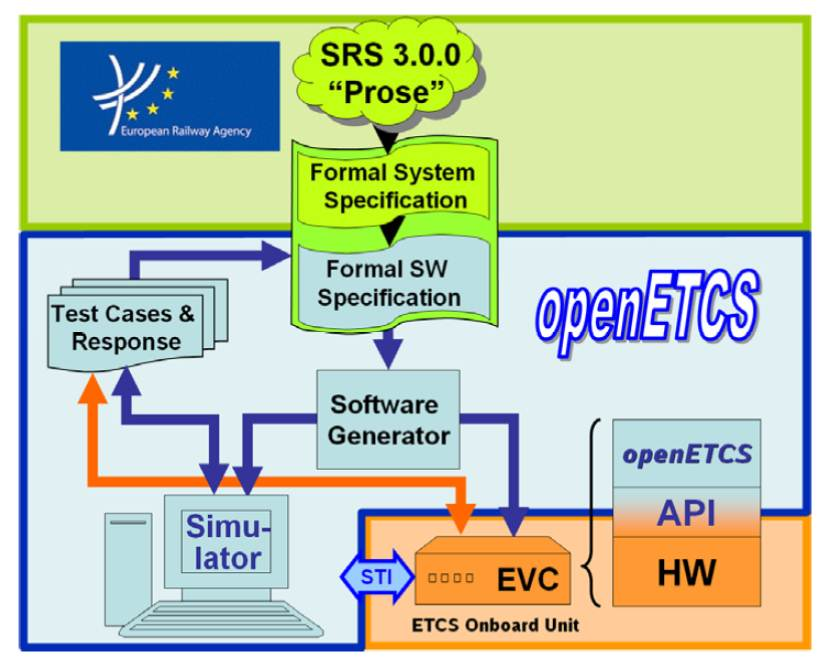
\includegraphics[width=12cm]{openETCS4}
%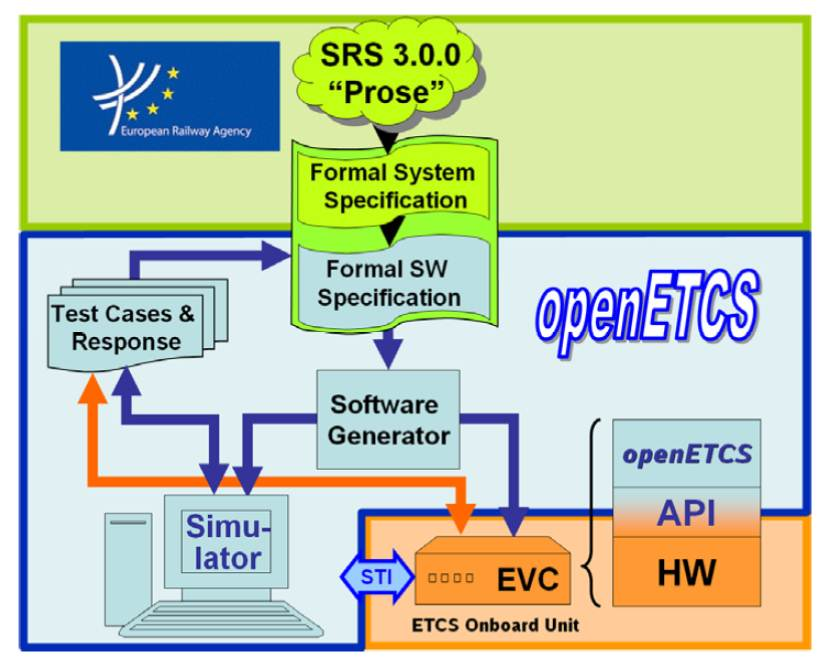
\includegraphics[width=1.0\textwidth, height=242px]{openETCS4}
\caption{the openETCS approach}
\label{fig:openETCS4}
\end{figure}


\chapter{Goal of the OpenETCS project}
\section{Description}
A detailed description of the openETCS project is given in the Project Outline Full Project
Proposal, see \cite{FPP13}.

\section{Main goals of the OpenETCS project}
\label{goals}
Generally, the overall goal of the openETCS project is to provide a usable open source application software; including tools, documentation and the safety case for all ETCS OBU. All these deliverables will be made available as FLOSS under a "General Public License" (e.g. EUPL: European Union Public License).
\\
A detailed description of the goals of the openETCS project is given in D2.3 \cite{D23}. In this section we only lists the main goals of the openETCS project:
\begin{enumerate}
  \item Create a semi-formal reference specification for the ETCS requirements and architecture, completed by strictly formal models of sub-parts,
  \item Define a safety case concept for the full model and apply it on a subset of the on-board unit,  
  \item Provide a tool chain and process/methodologies for developing an on-board software that can fulfil the CENELEC requirements for SIL4 software,
  \item Provide an executable software package generated from the specification of on-board ETCS.
\end{enumerate}


\chapter{Purpose and software assessment process}
\section{Purpose of this report}
Due to the particularity of the openETCS project and taking into account its goals, it should
be clarify in advance which requirements shall be fulfilled in order to be compliant with the
CENELEC standards, particularly the CENELEC standard EN 50128:2011. This work was carried out and coordinated by AEbt and the result is described in the next section. 
This document lists requirements that must be fulfilled in order to prove, that the openETCS project deliverables (as described in section \ref{goals}) are compliant with the above mentioned CENELEC standard.

\section{Realization of this report}
\label{report}
Basis for the realisation of this document were:
\begin{itemize}
  \item Articles and other technical literature
  \item Existing processes in the signalling industry
  \item CENELEC standards
\end{itemize}

This work was also carried out through interviews with experts. The experts interviewed were industrial experts, signalling experts and standardisation experts. 


\section{Assessment of safety related railway software}
A safety related railway software will pass the assessment process, if it has been proved that the actual behavior of the software during testing and validation was consistent with the behavioral semantic of the software. 
The behavioral semantic of a software is observable in: 
\begin{itemize}\itemsep=0pt
  \item The data domain,
  \item The time domain,
  \item The causal domain.
\end{itemize}

All the above mentioned behavioral aspects depend on both: the \textbf{operating system} (OS) and the underlying \textbf{Hardware} (HW). 
For example:
\begin{itemize}\itemsep=0pt
  \item Data transformations fail if, the word length of the HW registers is inappropriate for the calculations involved,
  \item Expected reactions miss their deadlines if, the OS scheduler does not allocate appropriate amounts of CPU time to the task processing the input,
  \item Events occur in the wrong order if the OS does not provide adequate mechanisms for critical section management,
  \item etc.
\end{itemize}

As a consequence a software is always assessed in relation with certain OS and HW resp. system capabilities.

The HW resp. system in which a safety related software shall be implemented, must be compliant with EN 50126 and EN 50129 (see \cite{EN50126}, \cite{EN50129}) depending on the resulting safety integrity levels from a prior performed hazard analysis and risk assessment.

When it is expected that the System in which a safety related software shall be implemented, exchanges safety-related data with its environment, the communication protocol must be compliant with EN 50159 (see \cite{EN50159}).

Concerning the OS, it is usual to elaborate specification documents about the OS capabilities required.

To reduce the complexity of the OS, the usual approach consists in creating an interface between the application software and the OS: the application program interface (API).
The API provides services necessary to ensure the proper behavior of the software to be executed. Concerning the safety integrity, the API must be compliant with EN 50128 (see \cite{EN50128}) depending on the application software SIL level and OS SIL level.


\chapter{Results}
\label{objective}
This section describes the result of the performed work.

\textbf{In summary:}
The first objective of the OpenETCS project is to get an unambiguously ERTMS OBU reference model. Getting such a reference model resulting from SSRS (as described in D2.6 \cite{D26}) and 100\% semi-formal, modelling of the SSRS, simulation and full validation of the Non-SIL generated code (with no class Tx code generator and compiler) will be performed.

The second objective of the OpenETCS project and so useful for future, is to define a safety process to be followed in order to get an EN 50128:2011 SIL4 verified code from the 100\% semi-formal model of the SSRS and apply this process on part of the SSRS to prove the integrity of this process.

Since for objective 1 no safety is required, no CENELEC Standards requirements need therefore to be fulfilled.

The results present in this chapter are only valid for objective 2


\section{Safety requirements to be fulfilled according to the CENELEC standards for objective 2}

Usually, the CENELEC standard EN 50128 is included in a top down workflow, starting with the EN 50126, EN 50129 and the EN 50159.
In fact the EN 50126 and the EN 50129 require that the following tasks are carried out:
\begin{itemize}
  \item identify hazards, assessing risks and arriving at decisions based on risk criteria,
  \item identify the necessary risk reduction to meet the risk acceptance criteria,
  \item define an overall System Safety Requirements Specification for the safeguards necessary to achieve the required risk reduction,
  \item select a suitable system architecture,
  \item plan, monitor and control the technical and managerial activities necessary to translate the System Safety.
\end{itemize}
Requirements Specification into a Safety-Related System of a validated safety integrity. As decomposition of the specification into a design comprising safety-related systems and components takes place, further allocation of safety integrity levels is performed. Ultimately this leads to the required software safety integrity levels.

In the case of openETCS: objective 2, we start at the end of the workflow, therefore safety related application conditions for the above elements (EN 50126 and EN 50129) must be defined.


\subsection{Requirements for the Software}
The CENELEC EN 50128:2011 requirements to be fulfilled are listes in appendix \ref{annexA} for tools and appendix \ref{annexB} for the software (openETCS application software and API).

\subsection{Requirements for the System and the Operating System}
Safety related application conditions for the system (HW) according to EN 50126 and EN 50129 and the OS according to EN 50128 must be defined and recorded.

\subsection{Requirements for the communication protocol (when applicable)}
Safety related application conditions for the communication protocol according to EN 50159 must be defined and recorded.



\section{Security requirements}
Besides safety resp. the functional safety, the security is becomming increasingly important in the use of safety related systems.
The success story of systems with open source software continues in the industrie, nevertheless these systems are more vulnerable to malicious attacks, sabotage or spionage. 
Until today, no standard has been established for security. However, according to the performed interviews, the IEC standard 62443 seem to be often used as the basis for tests again security.
we therefore recommend to elaborate safety related application conditions according to the IEC standard 62443 that must be fulfilled.


\section{Is "open proofs" suitable for safety related railway applications?}
As mentioned in section \ref{common-terms}; a software or system is an "open proofs" if all of the following are FLOSS: 
\begin{enumerate}
\itemsep=0pt
  \item the entire implementation (requirements, design, code, required documentation for use/maintenance, etc.),
  \item automatically-verifiable proof(s) of at least one key property, and
  \item all required tools needed for use and modification of the software or system.
\end{enumerate}

According to (http://www.openproofs.org), something is FLOSS if it gives anyone the freedom to use, study, modify, and redistribute modified and unmodified versions of it, meeting the free software definition and the open source definition.

In a globally meaning, "open Proofs" embraces two approaches: formal methods and the freely availability of the software or system to others (in this report referred as open source).


\subsection{Suitability of open source for safety related railway applications}
By order of the Deutsche Bahn AG (DB AG), AEbt has created an assessment report on the suitability of open source software for safety relevant railway applications.
In this Report, the assessor came to the conclusion that open source software regarding their safety integrity should be treated just as proprietary software. In certain areas, the use of open source software for safety relevant applications is even recommended; because software bugs or intentionally programmed backdoor will be early detected by independent programmers or the "community", see \cite{AEbt-doc}.


\subsection{Suitability of formal methods for safety releted railway applications}
This section provided general information of the impact of introducing and integrating formal methods (FM) into the development process.

Formal methods for developing software embrace two techniques: formal specification and formal verification. Both are established based on elementary mathematics, such as set of theory, logic and algebraic theory \cite{SOFL-doc}.

When establishing formal methods on a project, there are basically two types of considerations, one of which is largely administrative, the other largely technical, \cite{FM-doc}. 

A summary of the each appears below.

\textbf{Administrative Factors:}
\begin{itemize}\itemsep=0pt
  \item \textbf{Project Staffing:} The team responsible for planning the role of FM on a project should include at least one person knowledgeable in FM and one person knowledgeable about the application domain. The team responsible for applying FM must have FM expertise or be provided with hands-on training.
  \item \textbf{Project Scale:} The scale of the project should be taken into consideration. If project staff has little or no previous FM experience, an initial study may be advisable either as a final objective or as a leading to the full-scale project.
  \item \textbf{FM Training:} The training available to those project staff responsible for applying FM should be rigorous and include hands-on experience with the tool(s) and type of application that will be encountered on the project.
  \item \textbf{Process Integration:} The strategy for integrating FM into a new or existing process should be thoroughly planned and documented, preferably early in the project.
  \item \textbf{Project Guidelines:} Project guidelines, standards, and conventions, both for documentation and specification, should be developed early and adhered to.
\end{itemize}

\textbf{Technical Factors:}
\begin{itemize}\itemsep=0pt
  \item \textbf{Type of Application:} FM are not equally appropriate for all applications; they are best suited to analyzing complex problems, taken singly and in combination, and less suited for numerical algorithms or highly computational applications..
  \item \textbf{Size and Structure of Application:} The size and structure of an application determine the difficulty of using FM; ideally, applications should be of moderate size (guidance on how to assess size will be addressed in this item's section below), decomposable into subsystems or components, and based on a coherent underlying structure.
  \item \textbf{Type of Analysis/Formal Method:} The type of analysis, i.e., the reasons for applying FM, determine the most appropriate level of formalization and the most suitable FM and FM tools. Objectives in using FM range from producing clear, unambiguous documentation to mechanically verifying the correctness of crucial algorithms or components.
  \item \textbf{Levels of Rigor in FM:} FM may be applied at varying levels of rigor. The rigor, or extent to which a method is "truly formal" and "really calculates," can range from the occasional appearance of mathematical notation in an otherwise informal document, through "rigorous" methods that employ a standardized specification language, to "fully formal" methods that make use of mechanically-checked theorem proving.
  \item \textbf{Scope of Formal Method Use:} There are at least three dimensions to the scope of formal method use: (1) all/selected stages of development life cycle, (2) all/selected system components, (3) full/selected (system) functionality.
  \item \textbf{Type of Formal Method Tool:} The choice of FM tool, if any, should be directly determined by the application profile generated by evaluating the five preceding factors. Primary considerations include the type of specification language and the need for mechanical proof support.
\end{itemize}

Administrative and technical considerations are closely coupled, each having implications for the other. This is because the process of determining whether a given application is a good candidate for FM is not cut and dried and because the use of FM entails a serious technical commitment by project staff and a corresponding commitment to support and invest in the FM activity on the part of management. 


\subsubsection{Detailed description of the technical considerations}
Formal methods cover a wide range of techniques that have different characteristics and utility. This section describes the scope and implications of these differences with respect to five technical factors that should be evaluated when considering the use of FM for a given application. The factors are introduced in the suggested order of consideration (according to \cite{FM-doc}); e.g., before choosing a formal method tool, it is important, first, to define the type and scope of application, second, to specify the type of analysis to be performed and third, to determine the rigor and scope of the analysis.

\textbf{Type of Application}
FM are not equally suitable for all types of applications. Although, in principle, the methods can be applied to nearly any application, in practice, the benefits that can be realized and the difficulty of achieving them will differ significantly from one application to another and from one subsystem to another within a single application. Suitability should be evaluated with respect to the characteristics of the problem domain and their implications for the modeling domain. 
Higher complexity applications stand to gain from FM much more than lower complexity ones simply because less complex problems can be solved dependably using less rigorous methods. Of particular interest are problem domains whose complexity stems not so much from the size and structure of the design, but from inherently difficult algorithms such as those for fault tolerance and parallel or distributed processes. 
A further consideration is the mathematical domain of discourse. Applications that are heavily based on numerical processing, especially those using floating point arithmetic, pose some difficulties for FM, while those that can be modeled using the domains of logic and discrete mathematics benefit from easier formalization, more tractable reasoning, and better FM tool support.

\textbf{Size and Structure of Application}
The size of an application is a major factor in the cost and difficulty of its formalization. 
Usually, FM are most effectively applied to systems or subsystems of moderate size; currently, FM cannot be applied in full to the largest systems implementable using conventional programming techniques. An alternative is to limit the scope of the formal method activity to critical properties or components of a very large system, assuming, of course, that the system is decomposable into small or medium-sized subsystems or components with well-defined interfaces. This clean structuring property is vital in any medium- or large-scale application to ensure that the results of separate FM analyses can be combined and valid inferences drawn about the composite behavior of cooperating subsystems.
A second structural property, loosely referred to as structural entropy, is also important. If an application has intrinsically high entropy, i.e., is primarily a random collection of special cases with weak cohesion or few unifying principles, little can be expected from a formalization activity. Conversely, if an application exhibits strong underlying structural principles, well understood and easily expressed in a logically meaningful way, FM can effectively capture and exploit this structure.

\textbf{Type of Analysis/Formal Method }
The type of analysis or formal method to be employed is determined largely by project objectives; the purpose for which FM are to be applied should be clearly defined and explicitly documented. For example, one application may use FM primarily to develop specifications for documentation, another may exploit the precision inherent in formally specified requirements to catch errors early in the life cycle, a third may use FM to analyze and assure the correctness of critical properties or algorithms. These equally legitimate objectives have very different implications for the rigor of the formal method analysis and the type of formal method tool appropriate for the project.

\textbf{Levels of Rigor in Formal Methods }
FM techniques may be applied at varying levels of rigor. Here, rigor is used in a technical sense to mean the degree of formality of a method, i.e., the extent to which a method formulates specifications in an axiomatic style, explicitly enumerates all assumptions, and reduces proofs to explicit applications of elementary rules of inference. Increasing formality allows the products of FM (i.e., specifications and proofs) to be less dependent on subjective reviews and consensus and more amenable to systematic analysis and replication. Usually, increasing formality is associated with increasing dependence on mechanical support. Suggested levels of rigor according to \cite{FM-doc}
\begin{itemize}\itemsep=0pt
  \item \textbf{Level 1:} Use of manual review and inspection, relying on documents written in a natural language, pseudo code, or programming language, possibly augmented with diagrams and equations, and validated with conventional testing techniques. Activities at this level are not "formal" in a strict sense, but represent current recommended practice, and serve as a baseline of discipline and structure necessary to support the additional activities at higher levels of formality.
  \item \textbf{Level 2:} Use of notations and concepts derived from logic and discrete math to develop more precise requirements statements and specifications. Proof, if any, is informal. This level of FM typically augments existing processes without imposing wholesale revisions.
  \item \textbf{Level 3:} Use of formalized specification languages with mechanized support tools ranging from syntax checkers and pretty printers to type checkers. This level of formality usually includes support for modern software engineering constructs, e.g., modules, abstract data types, and objects, all with explicit interfaces, but has not historically offered mechanized theorem proving.
  \item \textbf{Level 4:} Use of fully formal specification languages with rigorous semantics and correspondingly formal proof methods that support mechanization. State exploration, model checking, and language inclusion technologies also exemplify this level, although these technologies are highly specialized, automatic theorem provers that are limited to checking properties of finite-state systems. 
\end{itemize}
Higher levels of rigor are not necessarily superior to lower levels; factors that determine the appropriate level of rigor include: project objectives, criticality of the application, and available resources. For example, if FM are used simply as documentation, Level 2 may be appropriate; if they are used to justify the design of a new and critical component, Level 4 may be the best choice. On the other hand, routine applications adequately handled by conventional processes are probably most appropriately left to Level 1. Finally, it is possible to use a formal method at a level of rigor lower than its ultimate capability, e.g., by using the specification language, but not the theorem-proving capability of a Level 4 formal method. 

\textbf{Scope of Formal Method Use}
The extent to which FM are applied can also vary. There are at least the following three dimensions to the notion of extent.
\begin{enumerate}\itemsep=0pt
  \item \textbf{All or selected stages of the development life cycle:} It is generally felt that the biggest payoff from the use of FM occurs in early life cycle stages, given that errors become more expensive to correct as they proceed undetected through later development stages; early detection leads to lower life cycle costs. Moreover, the use of FM in the early stages provides additional precision where it is currently most needed in the conventional development process.
  \item \textbf{All or selected system components:} Criticality assessments, assurance considerations, and architectural characteristics are among the key factors used to determine which subsystems or components to analyze with FM. Since large systems are typically composed of components with widely differing criticalities, the extent of formal method use should be dictated by project-specific criteria. For example, a system architecture that provides fault containment for a critical component through physical or logical partitioning provides an obvious focus for FM activity and enhances its ability to assure key system properties.
  \item \textbf{Full or selected system functionality:} Although FM have traditionally been associated with "proof of correctness," i.e., ensuring that a system component meets its functional specification, they can equally well be applied to only the most important system properties. Moreover, in some cases it is more important to ensure that a component does not exhibit certain negative properties or failures, rather than to prove that it has certain positive properties, including full functionality.
\end{enumerate}
These are the three most commonly used variations on the extent of FM application, although others are certainly possible. Varying the degree of rigor along each of these three dimensions yields a wide range of options and provides maximal benefit from a limited investment in FM.

\textbf{Type of Formal Method Tool}
The choice of tool is dictated by the application profile defined by consideration of all of the preceding factors, although the issue of tools is clearly moot if the most appropriate level of rigor falls below Level 3. For example, Level 3 documentation of sequential components is consistent either with a typical Level 3 notation supported by a type checker, or, if more powerful mechanization and stronger guarantees of consistency are desired, with a system normally used to support Level 4. Similarly, when choosing a Level 4 tool, the capability of the tool, the constraints of the problem domain, and the objectives of the analysis must be well matched. For example, verifying the correctness of fault-tolerant algorithms is probably best pursued with a general-purpose theorem prover, while exploring the properties of mode-switching or other complex control logic is probably more effectively pursued with a state-exploration system.
The process of selecting a formal method tool is in many ways similar to selecting any other software system; the usual considerations of documentation, tutorials, history of use, ease of use, etc. apply. In this case, effective support for the selected formal method(s) is also important. A suggestive, but by no means exhaustive, list of the additional considerations necessary for judicious tool selection appears below. 
\begin{enumerate}\itemsep=0pt
  \item \textbf{Specification Language:} Is the language adequately expressive for the given application and which of the following features important for the application does the language offer: well-defined semantics, modern programming language constructs (including support for abstraction, modularity, and encapsulation), familiar and convenient syntax, strong typing, encapsulation, parameterization, built-in model of computation, executable subset or other provision for animating specifications, support for state exploration, model checking, and related methods?
  \item \textbf{Theorem Prover:} Does the FM tool offer a theorem prover or proof checker? If so, how is the theorem prover controlled and guided; is there automated support for arithmetic reasoning, efficient handling of large propositional expressions, and rewriting; what support is there for developing and viewing the proof; how is the proof presented to the user (e.g., user input or canonical expressions, with or without quantifiers); are the foundations (i.e., all axioms, definitions, assumptions, lemmas) of the proof identified; are there facilities for editing proofs; is it reasonably easy to re-verify a theorem after slight changes to the specification?
  \item \textbf{Utilities:} Does the formal method offer a reasonably comprehensive library of standard types, functions, and other constructions and is the library validated; what, if any, editing and document preparation tools does the system provide; are there facilities for cross-referencing, browsing, and requirements tracing; is there support for incremental development across multiple sessions and for change control and version management?
\end{enumerate}


\subsection{Position of standards regarding formal methods in the railway sector}
In EN 50128:2011, Formal Methods/Proofs are explicitly identified as relevant technique/measure for software requirements specification, software architecture, software design, implementation, verification and testing and data preparation techniques. More precisely they are "recommended" for SIL levels 1 and 2 and "Highly Recommended" for SIL levels 3 and 4. The standard puts additional constraints on tools, especially code/data generation tools with respect to the need of a specification and evidence that the implementations complies with the specification. 
Unfortunately, formal methods have not spread in the whole railway signalling industries, where much software is still written and tested in traditional ways. This lack of adoption is due to the investments needed to build up a formal methods culture, and to the high costs of commercial support tools. Moreover, equipment can conform to CENELEC without applying formal methods \cite{Proc-doc}. 
Another barrier is that, the certification bodies might not be familiar with FM as most of the systems they certify follow a test-based approach. For systems whose justification relies on such formal argument, the certification body might require additional information to be convinced. Typically, one should foresee some specific training-level information in the certification process. Once acquired, new system can easily follow the same path. \linebreak \linebreak For example Siemens has gone through this process with the B-method, and it is now accepted by the certification bodies, so that the next projects have become easier to certify. 

\textbf{In summary:} The EN 50128:2011 highly recommend formal methods but do not really describe how to manage a formal development. Certification authorities have to be convinced about this issue. 
As formal methods are less widespread and certification authorities are less familiar with them as compared to the classical development methods, there is more work to be done in comparison with other methods, especially the first time, and despite the fact that better argument could be provided. However the investment might be worth the effort as shown by the Siemens case for B-method. 



\chapter{Summary}
As D2.2 task leader, AEbt has coordinated all the work. Basis for the creation of this document were the procedures listed in section \ref{report} of this document. The result is a set of requirements, which shall be fulfilled in order to reach objective 2 of the openETCS project (see chapter \ref{objective}). 

In this document reference was made to other CENELEC standards ( EN 50126 \cite{EN50126}, EN 50129 \cite{EN50129}, EN 50159 \cite{EN50159}); which however have not been detailed, but shall be considered in the openETCS safety case.

The opinions given in column "how the evidence shall be provided" in each table of the appendices \ref{annexA}and \ref{annexB} are just one of many possible solutions about how the corresponding requirement can be fulfilled.

Based on the performed assessment and interviews, we are of the opinion that "open proofs" is suitable for railway sector, when the process applied to developped the system and software fulfills the corresponding CENELEC requirements and also the security requirements (for example from the IEC 62443).



\nocite{*}

\bibliographystyle{unsrt}
\bibliography{erdc}

\appendix

\chapter{Requirements for tools}
\label{annexA}
This appendix lists requirements that tools shall fulfill within the openETCS project, in order to reach objective 2.

\section{Introduction}
The standard 50128:2011 distinguishes between three software tool classes (T1, T2 and T3). Therefore, this appendix  lists for each software tool class, the requirements to be fulfilled:
\begin{itemize}\itemsep=0pt
  \item Section \ref{T1}, lists requirements for tool in class T1,
  \item Section \ref{T2}, lists requirements for tool in class T2 and,
  \item Section \ref{T3}, lists requirements for tool in class T3.
\end{itemize}

\subsection{How to read the tables used in this appendix}
Tables used in this appendix consist of three columns.
\begin{itemize}\itemsep=0pt
  \item \textbf{Column 1} lists the requirements comming from the CENELEC standard EN 50128:2011. But since the standard is protected by copyright, only the requirements identification numbers are recorded there. The same requirements identification numbers (subclause) as defined in the EN 50128:2011 have been used. The textual requirement should therefore be read in the standard using the requirements identification number recorded in column 1 as reference.\\
In order to simplify the readability, some of the requirements have been grouped, especially when they address the same subject; only few were left out, because they were not relevant for the purpose.
  \item \textbf{column 2} gives one of many possible solutions about how the corresponding requirement can be fulfilled.
  \item \textbf{column 3} gives in which document the requirement shall be treated resp. the evidence document to be created or provided.
\end{itemize}


\section{Requirements for tools in class T1}
\label{T1}
Some examples of T1 tools:
\begin{itemize}\itemsep=0pt
  \item a text editor tool with no automatic code generation capabilities,
  \item a requirement support tool with no automatic code generation capabilities,
  \item a design support tool with no automatic code generation capabilities,
  \item configuration control tools.
\end{itemize}

{\footnotesize\sffamily\centering
\begin{longtable}{|p{2cm}|p{9cm}|p{3cm}|}
\caption{T1 tools safety proof}\\
\hline
\bfseries Requirements & \bfseries How the evidence shall be provided & \bfseries Evidence documents\\
\hline
\hline
\endhead
\hline
%\caption{Terms and definitions}
\endfoot

6.7.4.1 & Provided the evidence that openETCS T1 tools cooperate. \linebreak \linebreak \textit{(Tools cooperate if the outputs from one tool have suitable content and format for automatic input to a subsequent tool, thus minimizing the possibility of introducing human error in the reworking of intermediate results)}. & Provided a tool manual for each openETCS T1 tool \linebreak \linebreak \textit{(the tool manual shall clearly defines the behaviour of the tool and any instructions or constraints on its use)}. \\ 
\hline
6.7.4.10 & Each openETCS T1 tools must be subject to configuration management. & Define a configuration management process for openETCS tools.\\ 
\hline
\end{longtable}}


\section{Requirements for tools in class T2}
\label{T2}
Tools in class T2 are in general verification tools.\\
Some examples of T2 tools:
\begin{itemize}\itemsep=0pt
  \item static code analysers,
  \item test coverage monitors,
  \item theorem proving assistants,
  \item simulators and,
  \item model checkers.
\end{itemize}

{\footnotesize\sffamily\centering
\begin{longtable}{|p{2cm}|p{9cm}|p{3cm}|}
\caption{T2 tools safety proof}\\
\hline
\bfseries Requirements & \bfseries How the evidence shall be provided & \bfseries Evidence documents\\
\hline
\hline
\endhead
\hline
%\caption{Terms and definitions}
\endfoot

6.7.4.1 & Provided the evidence that openETCS T2 tools cooperate \linebreak \linebreak \textit{(Tools cooperate if the outputs from one tool have suitable content and format for automatic input to a subsequent tool, thus minimizing the possibility of introducing human error in the reworking of intermediate results)}. & See 6.7.4.3.\\ 
\hline
6.7.4.2 & Provided the evidence that failures in the output of each openETCS T2 tool are detected.& Provided a validation report for each openETCS T2 tool  \linebreak \linebreak \textit{(The validation report shall include the identification of potential failures which can be injected into the tools output and the measures to avoid or handle such failures)}.\\ 
\hline
6.7.4.3 & Provide a tool manual for each openETCS T2 tools. & Tool Manual for each openETCS T2 tool \linebreak \linebreak \textit{(the tool manual shall clearly defines the behaviour of the tool and any instructions or constraints on its use)}.\\ 
\hline
6.7.4.10 & Each openETCS T2 tools must be subject to configuration management. & Define a configuration management process for openETCS tools.\\ 
\hline
6.7.4.11 & For each new version of the openETCS T2 tools that is used, provide the evidence that the new version contains no significant new unknown faults. & Each Evidence in 6.7.4.2, 6.7.4.3 and 6.7.4.10 must be provided.\\ 
\hline
\end{longtable}}


\section{Requirements for tools in class T3}
\label{T3}
Some examples of T3 tools: 
\begin{itemize}\itemsep=0pt
  \item Design refinement tools,
  \item Compilers,
  \item Assemblers,
  \item linkers,
  \item binders,
  \item loaders,
  \item Code generation tools,
  \item Diagnostic tools used to maintain and monitor the software under operating conditions,
  \item Application data/algorithm tools.
\end{itemize}

{\footnotesize\sffamily\centering
\begin{longtable}{|p{2cm}|p{9cm}|p{3cm}|}
\caption{T3 tools safety proof}\\
\hline
\bfseries Requirements & \bfseries How the evidence shall be provided & \bfseries Documents to be created\\
\hline
\hline
\endhead
\hline
%\caption{Terms and definitions}
\endfoot

6.7.4.1 & Provide the evidence that openETCS T3 tools \linebreak \linebreak \textit{(Tools cooperate if the outputs from one tool have suitable content and format for automatic input to a subsequent tool, thus minimizing the possibility of introducing human error in the reworking of intermediate results)}. & See 6.7.4.3.\\ 
\hline
6.7.4.2 & Provided the evidence that failures in the output of each openETCS T3 tool are detected. & See 6.7.4.4.\\ 
\hline
6.7.4.3 & Provide a tool manual for each openETCS T3 tool. & Tool Manual for each openETCS T3 tool \linebreak \linebreak \textit{(the tool manual shall clearly defines the behaviour of the tool and any instructions or constraints on its use)}.\\
\hline
6.7.4.4 & Provided the evidence that the output of each openETCS T3 tool is conform to the specification of the output.& 
According to EN 50128:2011, the evidence may be based on one of the following topic:
\begin{enumerate}\itemsep=0pt
  \item a tool validation report as specified in 6.7.4.5,
  \item diverse redundant code which allows the detection and control of failures resulting in faults introduced by a tool,
  \item Compliance with the safety integrity levels derived from the risk analysis of the process,
\end{enumerate}\\ 
\hline
6.7.4.5 & Each validation report for a T3 tool must fulfill all the following requirements:
\begin{itemize}\itemsep=0pt
  \item a description of the validation activities;
  \item the version of the tool manual being used;
  \item the tool functions being validated;
  \item tools and equipment used;
  \item the results of the validation activity;
  \item test cases and their results for subsequent analysis;
  \item discrepancies between expected and actual results.
\end{itemize}
& tool validation report\\ 
\hline
6.7.4.10 & Each openETCS T3 tools must be subject to configuration management. & Define a configuration management process for openETCS tools.\\ 
\hline
6.7.4.11 & For each new version of the openETCS T3 tools that is used, provide the evidence that the new version contains no significant new unknown faults. & Each Evidence in 6.7.4.2, 6.7.4.3, 6.7.4.4 and 6.7.4.10 must be provided.\\ 
\hline
\end{longtable}}


\newpage
    
\section{Result}
According to the performed interviews with Esterel Technologies (Esterel Technologies has developed a T3 class tool for SIL4 application according to EN 50128:2011) and based on our resources; the openETCS team will not be able to develop all the T3 tool required within the context of the openETCS project. According to this, we recommend to define an automatic software verification process with openETCS T2 tools. The process shall describe and demonstrate, how to verify with openETCS T2 tools a software generated from a "non T3" code generator, so that at the end of the Verification, the verified code can be assessed as SIL4 verified code according to EN 50128:2011.



\chapter{Requirements for the software}
\label{annexB}
\section{Introduction}
This appendix lists requirement that the openETCS application software and API shall fulfill, in order to be compliant with CENELEC standard EN 50128:2011 for SIL4 Software (objective 2 of the openETCS project).

\subsection{How to read the tables used in this appendix}
Tables used in this appendix consist of three columns.
\begin{itemize}\itemsep=0pt
  \item \textbf{Column 1} lists the requirements comming from the CENELEC standard EN 50128:2011. But since the standard is protected by copyright, only the requirements identification numbers are recorded there. The same requirements identification numbers (subclause) as defined in the EN 50128:2011 have been used. The textual requirement should therefore be read in the standard using the requirements identification number recorded in column 1 as reference.\\
In order to simplify the readability, some of the requirements have been grouped, especially when they address the same subject; only few were left out, because they were not relevant for the purpose.
  \item \textbf{column 2} gives one of many possible solutions about how the corresponding requirement can be fulfilled.
  \item \textbf{column 3} gives in which document the requirement shall be treated resp. the evidence document to be created or provided.
\end{itemize}


\section{Software Safety Integrity Levels (Clause 4 according to EN 50128:2011)}
\label{clause42}
{\footnotesize\sffamily\centering
\begin{longtable}{|p{2cm}|p{9cm}|p{3cm}|}
\caption{Safety Integrity Levels activities}\\
\hline
\bfseries Requirements & \bfseries How the evidence shall be provided & \bfseries Evidence documents\\
\hline
\hline
\endhead
\hline
%\caption{Terms and definitions}
\endfoot

4.1 & Provided the documentation of the system in which the openETCS software will be integrated 
The following system documentation shall be provided:
\begin{enumerate}\itemsep=0pt
  \item a functional and interface description of the system;
  \item application conditions;
  \item configuration or architecture of the system;
  \item hazards to be controlled;
  \item safety integrity requirements;
  \item apportionment of requirements and allocation of SIL to software and hardware;
  \item timing constraints.
\end{enumerate} & See system documentation in column "How the evidence shall be provided"\\ 
\hline
\end{longtable}}


\section{Management and organisation (Clause 5 according to EN 50128:2011)}
\label{clause52}
\subsection{Organisation, Roles and Responsabilities}
\begin{flushleft}
The objective of this subclause is to ensure that all personnel who have responsibilities within the openETCS project are organised, empowered and capable to fulfill theirs responsibilities.
\end{flushleft}
{\footnotesize\sffamily\centering
\begin{longtable}{|p{2cm}|p{9cm}|p{3cm}|}
\caption{Organisation, Roles and Responsabilities safety proof}\\
\hline
\bfseries Requirements & \bfseries How the evidence shall be provided & \bfseries Evidence documents\\
\hline
\hline
\endhead
\hline
%\caption{Terms and definitions}
\endfoot

5.1.2.1 & Provided an EN ISO 9001 certification or the Evidence of a quality management process according to EN ISO 9001 for each organization. & The openETCS safety case shall demonstrate that the quality management process within the openETCS project is compliant with EN ISO 9001.\\ 
\hline
5.1.2.2 to 5.1.2.14 & The openETCS safety Plan shall implement these requirements.& openETCS safety Plan\\ 
\hline
\end{longtable}}


\subsection{Personnel Competence}
\begin{flushleft}
The objective of this subclause is to ensure that all personnel who have responsibilities within the openETCS project are competent to discharge those responsibilities by demonstrating the ability to perform relevant tasks correctly, efficiently and consistently to a high quality and under varying conditions.
\end{flushleft}
{\footnotesize\sffamily\centering
\begin{longtable}{|p{2cm}|p{9cm}|p{3cm}|}
\caption{Personnel competence safety proof}\\
\hline
\bfseries Requirements & \bfseries How the evidence shall be provided & \bfseries Evidence documents\\
\hline
\hline
\endhead
\hline
%\caption{Terms and definitions}
\endfoot

5.2.2.1 and 5.2.2.2 & The evidence that all personnel who have responsibilities within the openETCS project are competent to discharge those responsibilities shall be provided. 
\begin{enumerate}\itemsep=0pt
  \item The process of assigning roles to persons shall be described in the openETCS system safety plan;
  \item Roles as defined in the EN 50128:2011 may only be assigned to persons with appropriate key competencies (as defined also in EN 50128:2011). Where key competencies to fulfill a role are missing, trainings must be provided. Participation in trainings shall also be referenced in a management document.
\end{enumerate} & openETCS safety plan, openETCS management document.\\ 
\hline
5.2.2.3 and 5.2.2.4 & See 5.2.2.1 and 5.2.2.2 & 5.2.2.1 and 5.2.2.2\\ 
\hline
\end{longtable}}

\subsection{Lifecycle issues and documentation}
\label{SDLC2}
\begin{flushleft}
The objective of this subclause is to structure the development process of the openETCS software into defined phases and activities and to record all information pertinent to the software throughout the lifecycle of the software.
\end{flushleft}
{\footnotesize\sffamily\centering
\begin{longtable}{|p{2cm}|p{9cm}|p{3cm}|}
\caption{Lifecycle issues and documentation safety proof}\\
\hline
\bfseries Requirements & \bfseries How the evidence shall be provided & \bfseries Documents to be created\\
\hline
\hline
\endhead
\hline
%\caption{Terms and definitions}
\endfoot

5.3.2.1 & Select a lifecycle model for the development of software and describe it in the openETCS quality assurance plan.
& openETCS software lifecycle model.\\ 
\hline
5.3.2.2 & See requirement 5.3.2.14 & See requirement 5.3.2.14\\ 
\hline
5.3.2.3 & openETCS Quality Assurance procedures shall run in parallel with lifecycle activities and use the same terminology. & Recommendation.\\ 
\hline
5.3.2.4 & The openETCS software Quality Assurance Plan, openETCS software V\&V Plan, openETCS software Maintenance Plan and openETCS software Configuration Management Plan shall be drawn up at the start of the openETCS project and maintained throughout the development life cycle of the project & Recommendation\\ 
\hline
5.3.2.5 & See requirement 5.3.2.14 & See requirement 5.3.2.14\\
\hline
5.3.2.6 & Requirement shall be implemented in the  openETCS quality assurance plan & openETCS quality assurance plan\\ 
\hline
5.3.2.7 & A traceability process shall be defined and referenced in the openETCS quality assurance plan. The defined traceability process shall implement this requirement.& openETCS traceability process\\ 
\hline
5.3.2.8 & Create a general openETCS glossary & openETCS glossary.
\linebreak
\linebreak
NOTE\linebreak
The created openETCS glossary shall be referenced in the openETCS software quality assurance plan.\\ 
\hline
5.3.2.9 & The section: "Documentation structure" of the openETCS software quality assurance plan shall implement this requirement. & openETCS software quality assurance plan, section "Documentation structure".\\ 
\hline
5.3.2.10 & Requirement shall be implemented in the  openETCS quality assurance plan & openETCS quality assurance plan\\ 
\hline
5.3.2.11 & Use well-established document file formats (html, ps, pdf, rtf, odf or latex).
& The selected file formats shall be recorded in the openETCS software quality assurance plan.
\linebreak
\linebreak
\textbf{Recommendation}\linebreak
The openETCS tools shall generate documents in file formats (pdf or office binary file formats)\\ 
\hline
5.3.2.12 and 5.3.2.13 & We do not recommend to combine documents created by independent roles. 
& - \\ 
\hline
5.3.2.14 & Where any alternative lifecycle or documentation structure is adopted, the evidence that the alternative lifecycle or documentation structure fulfill all the objectives and requirements of the CENELEC EN 50128:2011 must be provided.
\linebreak
\linebreak
NOTE\linebreak
For the selected alternative lifecycle, the Evidence may be based on the following topic:
\begin{itemize}\itemsep=0pt
  \item top-down design methods,
  \item possibility of iterations in and between phases
  \item modularity,
  \item verification of each phase of the development lifecycle,
  \item validation,
  \item Planning (All activities to be performed during a phase shall be defined and planned prior to the commencement of the phase),
  \item appropriate consideration of organisation and personnel competency issues.
\end{itemize}


For the selected alternative documentation structure,the Evidence  may be based on the following topic:
\begin{itemize}\itemsep=0pt
  \item clear documentation and traceability,
  \item auditable documents,
\end{itemize}
& The Evidence shall be described in the openETCS safety case.\\ 
\hline
\end{longtable}}



\section{Software assurance (Clause 6 according to EN 50128:2011)}
\label{clause62}
\subsection{Software Testing}
\begin{flushleft}
The objective of this subclause is to ascertain the behaviour or performance of the developed openETCS software against the corresponding test specification to the extent achievable by the test coverage.
\end{flushleft}
{\footnotesize\sffamily\centering
\begin{longtable}{|p{2cm}|p{9cm}|p{3cm}|}
\caption{Software Testing activities}\\
\hline
\bfseries Requirements & \bfseries How the evidence shall be provided & \bfseries Evidence documents\\
\hline
\hline
\endhead
\hline
%\caption{Terms and definitions}
\endfoot

6.1.4.1 to 6.1.4.4 and 8.4.8.6 & openETCS Test Specifications shall be created according to requirements 6.1.4.4 and 8.4.8.6.
& All Created openETCS Test Specifications shall be referenced in the openETCS Test plan or openETCS V\&V Plan\\ 
\hline
6.1.4.5 & After each performed Test, a test report shall be written. 
Each openETCS Test report shall be written according to requirement 6.1.4.5.
& This requirement shall be recorded in the openETCS Test plan or openETCS V\&V Plan\\ 
\hline
\end{longtable}}


\subsection{Software Verification}
\begin{flushleft}
The objective of this subclause is to examine and arrive at a judgment based on evidence that output of each development phase fulfill the requirements and plans with respect to completeness, correctness and consistency.
\end{flushleft}
{\footnotesize\sffamily\centering
\begin{longtable}{|p{2cm}|p{9cm}|p{3cm}|}
\caption{Software Verification activities}\\
\hline
\bfseries Requirements & \bfseries How the evidence shall be provided & \bfseries Evidence documents\\
\hline
\hline
\endhead
\hline
%\caption{Terms and definitions}
\endfoot

6.2.4.1 to 6.2.4.9 and 8.4.8.6 & An openETCS software verification plan shall be created according to requirements 6.2.4.9 and 8.4.8.6.

\textit{NOTE: \linebreak The appropriate combinations of techniques for software SIL4 as described in tables A.5, A,6, A.7 and A.8 of EN 50128:2011 shall be selected and recorded in the openETCS software verification plan.}
& openETCS V\&V Plan\\ 
\hline
6.2.4.10 to 6.2.4.11 & The created openETCS V\&V Plan shall be verify according to the requirement 6.2.4.11. 
The results of the verification shall be recorded in the openETC software quality assurance verification report.
& openETCS software quality assurance verification report.\\ 
\hline
6.2.4.12 to 6.2.4.13 & After each performed Verification, a verification report must be created. 
Test verification report shall be created according to requirement 6.2.4.13.
& This requirement shall be recorded in the openETCS V\&V Plan.\\ 
\hline
\end{longtable}}



\subsection{Software Validation}
\begin{flushleft}
The objective of this subclause is to determine whether the developed openETCS software fits the user needs, in particular with respect to safety and quality and with emphasis on the suitability of its operation in accordance to its purpose in its intended environment.
\end{flushleft}
{\footnotesize\sffamily\centering
\begin{longtable}{|p{2cm}|p{9cm}|p{3cm}|}
\caption{Software Validation activities}\\
\hline
\bfseries Requirements & \bfseries How the evidence shall be provided & \bfseries Evidence documents\\
\hline
\hline
\endhead
\hline
%\caption{Terms and definitions}
\endfoot

6.3.4.1 to 6.3.4.6 and 8.4.8.6 & A Software validation plan shall be created according to requirements 6.3.4.4 and 8.4.8.6.
& openETCS V\&V Plan \\ 
\hline
6.3.4.7 to 6.3.4.11 & After the validation of the "overall" software, a software validation report shall be created according to requirements 6.3.4.8 to 6.3.4.11
& This requirement shall be recorded in the openETCS V\&V Plan.\\ 
\hline
6.3.4.13 and 6.3.4.14 & The created openETCS V\&V Plan and openETCS software validation report shall be verify according to requirements 6.3.4.13 and 6.3.4.14. 
The results of the verification shall be recorded in the openETCS Software validation plan verification report. & openETCS Software validation plan verification report.\\ 
\hline
\end{longtable}}


\subsection{Software Assessment}
\textbf{These activities are not in the scope of the openETCS project and will be carried out by an independent safety assessor.}


\subsection{Software Quality assurance}
\begin{flushleft}
The objective of this subclause is to identify, monitor and control all those activities, both technical and managerial, which are necessary to ensure that the developed openETCS software achieves the quality required. 
\end{flushleft}
{\footnotesize\sffamily\centering
\begin{longtable}{|p{2cm}|p{9cm}|p{3cm}|}
\caption{Software Quality assurance activities}\\
\hline
\bfseries Requirements & \bfseries How the evidence shall be provided & \bfseries Evidence Documents\\
\hline
\hline
\endhead
\hline
%\caption{Terms and definitions}
\endfoot

6.5.4.1 & See requirement 5.3.2.4 & See requirement 5.3.2.4\\ 
\hline
6.5.4.2 & See requirement 5.3.2.1 & See requirement 5.3.2.1\\ 
\hline
6.5.4.3 to 6.5.4.6 & For the openETCS project a software quality assurance plan shall be created according (at least) to requirement 6.5.4.5.
& openETCS Software quality assurance.\\ 
\hline
6.5.4.7 to 6.5.4.8 & The created openETCS software quality assurance plan shall be verified according to requirement 6.5.4.8. 
The results of the verification shall be recorded in the openETCS Software quality assurance verification report.
& openETCS Software quality assurance verification report.\\ 
\hline
6.5.4.9 & The openETCS software Quality Assurance Plan, openETCS software V\&V Plan, openETCS software Maintenance Plan and openETCS software Configuration Management Plan shall have a paragraph specifying details about its own updating throughout the project: frequency, responsibility, method. & Highly Recommended\\ 
\hline
6.5.4.10 to 6.5.4.12 and 9.1.4.14 & A configuration management process for the openETCS project shall be defined and described in the openETCS configuration management plan.
The openETCS configuration management process shall be created according to requirements 6.5.4.10, 6.5.4.11, 6.5.4.12 and 9.1.4.14. 
& openETCS Software configuration management plan.\\ 
\hline
6.5.4.13 & See subclause 6.2 & See subclause 6.2\\ 
\hline
6.5.4.14 to 6.5.4.17 and 9.1.4.19 & The openETCS traceability process defined in subclause 5.3.2.7, shall also implement these requirements.
& openETCS traceability process.\\ 
\hline
\end{longtable}}


\subsection{Software Modification and change control}
\begin{flushleft}
The objective of this subclause is to ensure that the openETCS software performs as required, preserving the software safety integrity and dependability when modifying the software.
\end{flushleft}
{\footnotesize\sffamily\centering
\begin{longtable}{|p{2cm}|p{9cm}|p{3cm}|}
\caption{Software Modification and change control activities}\\
\hline
\bfseries Requirements & \bfseries How the evidence shall be provided & \bfseries Evidence Documents\\
\hline
\hline
\endhead
\hline
%\caption{Terms and definitions}
\endfoot

6.6.4.1, 6.6.4.2 and 8.4.8.5 & A change management process for the openETCS project shall be defined according to requirements from 6.6.4.1 to 6.6.4.2 and 8.4.8.5 and described in a  software change management plan 
& openETCS Software change Management Plan\\ 
\hline
\end{longtable}}


\subsection{Support tools and languages}
\begin{flushleft}
The objective of this subclause is to provide evidence that potential failures of tools do not adversely affect the integrated toolset output in a safety related manner that is undetected by technical and/or organisational measures outside the tool.
\end{flushleft}
{\footnotesize\sffamily\centering
\begin{longtable}{|p{2cm}|p{9cm}|p{3cm}|}
\caption{Support tools and languages for the development of the openETCS software}\\
\hline
\bfseries Requirements & \bfseries How the evidence shall be provided & \bfseries Evidences Documents\\
\hline
\hline
\endhead
\hline
%\caption{Terms and definitions}
\endfoot

6.7.4.1 to 6.7.4.11 & openETCS tools shall be used the development of the openETCS software & See appendix \ref{annexA}\\ 
\hline
\end{longtable}}



\section{Generic openETCS Software development (Clause 7 according to EN 50128:2011)}
\label{clause72}
\subsection{Lifecycle and documentation regarding the development of the openETCS software}
See Subsection \ref{clause52}.


\subsection{Software Requirements}
\label{req-sw}
\begin{flushleft}
The objective of this subclause is to describe a complete set of requirements for the openETCS software meeting all safety requirements and provides a comprehensive set of documents for each subsequent phase and to describe the overall test specification of the openETCS software.
\end{flushleft}
{\footnotesize\sffamily\centering
\begin{longtable}{|p{2cm}|p{9cm}|p{3cm}|}
\caption{openETCS Software requirements activities}\\
\hline
\bfseries Requirements & \bfseries How the evidence shall be provided & \bfseries Evidence Documents\\
\hline
\hline
\endhead
\hline
%\caption{Terms and definitions}
\endfoot

7.2.4.1 to 7.2.4.14 and 8.4.8.2 & The openETCS software requirements specification shall be written according to requirement 7.2.4.2 to 7.2.4.15 and 8.4.8.2.& openETCS software Requirements specification.
\linebreak
\linebreak
NOTE: \linebreak
The traceability of the openETCS software requirements specification back to the systems documents (System Requirements Specification, System Safety Requirements Specification, System Architecture Description, External Interface Specifications) is mandatory.\\
\hline
7.2.4.15 & The Selected techniques in Table A.2 of EN 50128:2011 shall be suitable for software SIL4.
& Record the selected techniques in the openETCS safety plan.\\ 
\hline
7.2.4.16, 7.2.4.17 and 7.2.4.19 & The overall Test Specification to test the openETCS "overall" software shall be written according to requirements 6.1.4.4 and 7.2.4.19. & openETCS overall software Test Specification\\ 
\hline
7.2.4.18 & The Selected techniques in Table A.7 of EN 50128:2011 shall be suitable for software SIL4. & The selected techniques shall be recorded in the openETCS V\&V Plan.\\ 
\hline
7.2.4.21 and 7.2.4.22 & The created openETCS software Requirements specification shall be verified according to requirements 7.2.4.22. 
The results of the verification shall be recorded in the openETCS software requirements verification report.
& openETCS software requirements verification report.\\ 
\hline
\end{longtable}}


\subsection{Software Architecture and Design}
\label{arc-sw}
\begin{flushleft}
The objective of this subclause is to develop an architecture of the openETCS software that achieves the requirements of the software and to identify and evaluate the significance of the interactions of the openETCS software with the hardware.
\end{flushleft}
{\footnotesize\sffamily\centering
\begin{longtable}{|p{2cm}|p{9cm}|p{3cm}|}
\caption{openETCS Software Architecture and Design activities}\\
\hline
\bfseries Requirements & \bfseries How the evidence shall be provided & \bfseries Evidence Documents\\
\hline
\hline
\endhead
\hline
%\caption{Terms and definitions}
\endfoot

7.3.4.1 to 7.3.4.15 & The openETCS software architecture specification shall be written according to requirement 7.3.4.2 to 7.3.4.15.& openETCS software architecture specification
\linebreak
\linebreak
NOTE: \linebreak
The traceability of the openETCS software architecture specification back to the openETCS software requirements specification is mandatory.\\ 
\hline
7.3.4.14 & The Selected techniques in Table A.3 of EN 50128:2011 shall be suitable for software SIL4.
& The selected techniques shall be recorded in the openETCS safety plan.\\
\hline
7.3.4.16 and 7.3.4.17 & Prototyping may be used in any phase to elicit requirements or to obtain a more detailed view on requirements and their consequences.& Recommendation\\ 
\hline
7.3.4.18, 7.3.4.19 and 8.4.8.3 & The openETCS software interface specification shall be written according to requirement 7.3.4.18, 7.3.4.19 and 8.4.8.3. & openETCS software interface specification.\\ 
\hline
7.3.4.20 to 7.3.4.23, 7.3.4.28, 8.4.8.7, 9.1.4.10, 9.1.4.13, 9.1.4.16 and 9.1.4.20
& The openETCS software design specification shall be created according to requirement 7.3.4.20 to 7.3.4.24, 7.3.4.28, 8.4.8.7, 9.1.4.10, 9.1.4.13, 9.1.4.16 and 9.1.4.20. & openETCS software design specification.\\
\hline
7.3.4.24 & The Selected techniques in Table A.4 of EN 50128:2011 shall be suitable for software SIL4.
& The selected techniques shall be recorded in the openETCS safety plan.\\ 
\hline
7.3.4.25 to 7.3.4.27 & A Coding standard used for the development of the openETCS software shall be suitable for software SIL4 .
\linebreak
The Coding standard used, shall include appropriate techniques in Table A.12 of EN 50128:2011 required for software SIL4.
& 
highly recommended.
\linebreak
\textbf{NOTE:} \linebreak
The coding standards used within the scope of the openETCS project shall be referenced in the openETCS software quality assurance plan.\\ 
\hline
7.3.4.29 and 7.3.4.31 & the openETCS software integration Test Specification for software integration testing shall be written according to requirements 6.1.4.4 and 7.3.4.31. & openETCS software integration Test Specification.\\ 
\hline
7.3.4.32 & The Selected techniques in Table A.5 of EN 50128:2011 shall be suitable for software SIL4.
& The selected techniques shall be recorded in the V\&V plan.\\ 
\hline
7.3.4.33 to 7.3.4.38 & The openETCS software/hardware integration Test Specification for software/hardware integration testing shall be written according to requirements 6.1.4.4 and 7.3.4.34. & openETCS software/hardware integration Test Specification.\\ 
\hline
7.3.4.39 & The Selected techniques in Table A.5 of EN 50128:2011 shall be suitable for software SIL4.
& The selected techniques shall be recorded in the V\&V plan.\\ 
\hline
7.3.4.40 to 7.3.4.43 & All the documents created in this phase (openETCS software architecture Specification, openETCS software interface Specification, openETCS software Design Specification,  openETCS software integration test specification and  openETCS software/hardware integration test specification)shall be verified according to requrements 7.3.4.40 to 7.3.4.43.
The results of the verification shall be recorded in the openETCS software architecture and design verification report. & openETCS software architecture and design verification report.\\ 
\hline
\end{longtable}}



\subsection{Software Component design}
\begin{flushleft}
The objective of this subclause is to develop and design software component that achieves the requirements of the openETCS software design specification to the extent required by the software safety integrity level.
\end{flushleft}
{\footnotesize\sffamily\centering
\begin{longtable}{|p{2cm}|p{9cm}|p{3cm}|}
\caption{openETCS software Component design activities}\\
\hline
\bfseries Requirements & \bfseries How the evidence shall be provided & \bfseries Evidence Documents\\
\hline
\hline
\endhead
\hline
%\caption{Terms and definitions}
\endfoot

7.4.4.1 to 7.4.4.5 & The openETCS software component Specification shall be created according to requirement 7.4.4.1 to 7.4.4.6. & openETCS software component Specification.
\linebreak
\linebreak
NOTE: \linebreak
The traceability of the openETCS software component Specification back to openETCS software architecture specification and openETCS software design specification is mandatory.\\ 
\hline
7.4.4.6 & The Selected techniques in Table A.4 of EN 50128:2011 shall be suitable for software SIL4.
& The selected techniques shall be recorded in the openETCS safety plan.\\ 
\hline
7.4.4.7 to 7.4.4.9 & The openETCS software component Test Specification shall be written according to the requirements 6.1.4.4 and 7.4.4.8 to 7.4.4.10.
& openETCS software component Test Specification.\\ 
\hline
7.4.4.10 & The Selected techniques in Table A.5 of EN 50128:2011 shall be suitable for software SIL4.
& The selected techniques shall be recorded in the V\&V plan.\\ 
\hline
7.4.4.11 to 7.4.4.13 & All the documents created in this phase (openETCS software component Specification and  openETCS component test specification)shall be verified according to requrements 7.4.4.11 to 7.3.4.13.
The results of the verification shall be recorded in the openETCS software component design verification report. & openETCS software component design verification report.\\ 
\hline
\end{longtable}}


\subsection{Software component implementation and testing}
\begin{flushleft}
The objective of this subclause is to achieve software component which is analysable, testable, verifiable and maintainable. This phase also include component testing.
\end{flushleft}
{\footnotesize\sffamily\centering
\begin{longtable}{|p{2cm}|p{9cm}|p{3cm}|}
\caption{openETCS Software component implementation and testing activities}\\
\hline
\bfseries Requirements & \bfseries How the evidence shall be provided & \bfseries Evidence Documents\\
\hline
\hline
\endhead
\hline
%\caption{Terms and definitions}
\endfoot

7.5.4.1 to 7.5.4.3 & The generated openETCS software component source code shall be compliant with the requirements 7.5.4.2 and 7.5.4.3.
& openETCS software component source code.\\ 
\hline
7.5.4.4 & Each generated openETCS software component source code shall be placed under configuration control before the commencement of testing.& Highly recommended.\\ 
\hline
7.5.4.5 to 7.5.4.7 & For each performed component test, a component test report shall be written. Each openETCS software component test report shall be written according to the requirements 6.1.4.5 and 7.5.4.6 to 7.5.4.7. & This requirement shall be recorded in the V\&V Plan\\ 
\hline
7.5.4.8 to 7.5.4.10 & Each generated openETCS software component source code shall be verified according to the requirements 7.4.4.11 to 7.3.4.13.
The results of each verification shall be recorded in the openETCS Software component verification report (according to 7.5.4.5 to 7.5.4.7).
& openETCS Software component verification.\\ 
\hline
\end{longtable}}



\subsection{Software Integration}
\begin{flushleft}
The objective of the openETCS software integration is to carry out openETCS software and software/hardware integration and demonstrate that the openETCS software and the hardware interact correctly to perform their intended functions.
\end{flushleft}
{\footnotesize\sffamily\centering
\begin{longtable}{|p{2cm}|p{9cm}|p{3cm}|}
\caption{openETCS Software Integration activities}\\
\hline
\bfseries Requirements & \bfseries How the evidence shall be provided & \bfseries Evidence Documents\\
\hline
\hline
\endhead
\hline
%\caption{Terms and definitions}
\endfoot

7.6.4.3 to 7.6.4.5 & Perform an integration tests of all openETCS software component.
After the performed integration tests of all openETCS software component, the openETCS Software integration test report shall be written. 
The openETCS Software integration test report shall be written according to the requirements 6.1.4.5 and 7.6.4.5. & openETCS Software integration test report.\\ 
\hline
7.6.4.7 to 7.6.4.9 & Perform a software/hardware integration test.
After the performed software integration test, the openETCS Software/hardware integration test report shall be written. 
The openETCS Software/hardware integration test report shall be written according to the requirements 6.1.4.5 and 7.6.4.9. & openETCS Software/hardware integration test report.\\ 
\hline
7.6.4.11 to 7.6.4.13 & All the documents created in this phase (openETCS Software integration test report and  openETCS Software/hardware integration test report)shall be verified according to requrements 7.6.4.11 to 7.6.4.13.
The results of the verification shall be recorded in the openETCS Software integration verification report. & openETCS Software integration verification report.\\ 
\hline
\end{longtable}}


\subsection{Software Validation}
\label{ValSW}
\begin{flushleft}
The objective of the software validation is to analyse and test the integrated openETCS software and hardware to ensure compliance with the software requirements specification with particular emphasis on the functional and safety aspects according to software SIL level and to check whether it is fit for its intended application.
\end{flushleft}
{\footnotesize\sffamily\centering
\begin{longtable}{|p{2cm}|p{9cm}|p{3cm}|}
\caption{openETCS Software Validation activities}\\
\hline
\bfseries Requirements & \bfseries How the evidence shall be provided & \bfseries Evidence Documents\\
\hline
\hline
\endhead
\hline
%\caption{Terms and definitions}
\endfoot

7.7.4.1 to 7.7.4.4 & Perform test of the overall openETCS software.
After the performed test of the overall openETCS software, the openETCS overall software test report shall be written. 
The openETCS overall software test report shall be written according to the requirement 6.1.4.5. & openETCS overall software test report.\\ 
\hline
7.7.4.6 to 7.7.4.11 & Perform a validation of the overall openETCS software.
After the performed validation of the overall openETCS software, the openETCS Software validation report shall be written. 
The openETCS Software validation report shall be written according to the requirements 7.7.4.6 to 7.7.4.11. & openETCS Software validation report.\\ 
\hline
7.7.4.12, 8.4.8.8, 9.1.4.4 and 9.1.4.5 & A Release Note which accompanies the delivered openETCS software shall be written according to requirements of 7.7.4.12, 8.4.8.8, 9.1.4.4 and 9.1.4.5.
& openETCS software release note.\\ 
\hline
\end{longtable}}




\section{Development of application data or algorithms (Clause 8 according to EN 50128:2011)}
\label{clause82}
\begin{flushleft}
The EN 50128:2011 considers that modern application design often makes use of generic software that is suitable as a basis for various applications. Such generic software is then configured by data, algorithms, or both, for producing the executable software for the application. The general Clauses 1 to 6 and 9 of the EN 50128:2011 apply to generic software as well as for application data or algorithms. The specific Clause 7 applies only for generic software while Clause 8 provides the specific requirements for application data or algorithms.
\end{flushleft}
\begin{flushleft}
\textit{\textbf{NOTE: }}
Clause 8 shall only be considered, if applicable for the openETCS project.
\end{flushleft}
\subsection{Application Data Development Process}
{\footnotesize\sffamily\centering
\begin{longtable}{|p{2cm}|p{9cm}|p{3cm}|}
\caption{openETCS Application Data Development Process activities}\\
\hline
\bfseries Requirements & \bfseries How the evidence shall be provided & \bfseries Evidence Document\\
\hline
\hline
\endhead
\hline
%\caption{Terms and definitions}
\endfoot

8.4.1.2 to 8.4.1.11 and 8.4.4.1 & The application preparation plan for the instantiation of the generic openETCS software shall be written according to requirements 8.4.1.2 to 8.4.1.11 and 8.4.4.1
& openETCS Application data preparation plan.\\ 
\hline
8.4.1.12 to 8.4.1.13 & The created openETCS Application data preparation plan shall be verified according to requrement 8.4.1.13.
The results of the verification shall be recorded in the openETCS application data verification report. & openETCS application data verification report.\\ 
\hline
\end{longtable}}


\subsection{Application Data Requirements Specification}
{\footnotesize\sffamily\centering
\begin{longtable}{|p{2cm}|p{9cm}|p{3cm}|}
\caption{openETCS Application Data Requirements Specification activities}\\
\hline
\bfseries Requirements & \bfseries How the evidence shall be provided & \bfseries Evidence Documents\\
\hline
\hline
\endhead
\hline
%\caption{Terms and definitions}
\endfoot

8.4.2.1 to 8.4.2.3 & The Application Data Requirements Specification shall be written according to requirements 8.4.2.1 to 8.4.2.3. & openETCS application data requirements specification.\\ 
\hline
8.4.2.4 and 8.4.2.5 & The created openETCS application data requirements specification shall be verified according to requrement 8.4.2.5.
The results of the verification shall be recorded in the openETCS application data verification report. & openETCS application data verification report.\\ 
\hline
\end{longtable}}


\subsection{Application Data Architecture and Design}
{\footnotesize\sffamily\centering
\begin{longtable}{|p{2cm}|p{9cm}|p{3cm}|}
\caption{openETCS Application Data Architecture and Design activities}\\
\hline
\bfseries Requirements & \bfseries How the evidence shall be provided & \bfseries Evidence Documents\\
\hline
\hline
\endhead
\hline
%\caption{Terms and definitions}
\endfoot

8.4.3.1  & The quantity and type of the generic hardware and software components to be used in the specific application shall be specified. The location of components, application data and algorithms in the specific application architecture shall be defined. The application data and algorithms processed by the generic software shall be designed at this stage.
& Highly recommended.\\ 
\hline
\end{longtable}}


\subsection{Application Data Production}
{\footnotesize\sffamily\centering
\begin{longtable}{|p{2cm}|p{9cm}|p{3cm}|}
\caption{openETCS Application Data Production activities}\\
\hline
\bfseries Requirements & \bfseries How the evidence shall be provided & \bfseries Evidence Documents\\
\hline
\hline
\endhead
\hline
%\caption{Terms and definitions}
\endfoot

8.4.4.3 & After performed Test of each application data component, an openETCS application data test report shall be created.
The openETCS application data test report shall be written according to requirement 6.1.4.5. & openETCS application data test report.\\ 
\hline
8.4.4.4 & After Verification of each application data component, an openETCS application data preparation verification report shall be created.
The openETCS application data preparation verification report shall be written according to requirement 8.4.4.4. & openETCS application data preparation verification report.\\ 
\hline
8.4.4.5 and 8.4.4.6 & To Test application data, an openETCS application data Test Specification shall be written.
The openETCS Application data Test Specification shall be written according to requirement 8.4.4.6. & openETCS Application data Test Specification.\\ 
\hline
8.4.4.7 and 8.4.4.8 & The created openETCS Application data Test Specification shall be verified according to requrement 8.4.4.8.
The results of the verification shall be recorded in the openETCS Application Data Verification Report. & openETCS Application Data Verification Report.\\ 
\hline
\end{longtable}}


\subsection{Data Integration and Testing Acceptance}
{\footnotesize\sffamily\centering
\begin{longtable}{|p{2cm}|p{9cm}|p{3cm}|}
\caption{openETCS Application Data Integration and Testing Acceptance activities}\\
\hline
\bfseries Requirements & \bfseries How the evidence shall be provided & \bfseries Evidence Documents\\
\hline
\hline
\endhead
\hline
%\caption{Terms and definitions}
\endfoot

8.4.5.1 and 8.4.5.2 & All tested application data component must now be integrated and tested again. To perform this task, a test specification shall be written according to requirement 8.4.5.2 . & openETCS application data test specification.\\ 
\hline
8.4.5.3 and 8.4.5.4 & The created openETCS application data test specification shall be verified according to requrement 8.4.5.4.
The results of the verification shall be recorded in the openETCS application data verification report. & openETCS Application Data Verification Report.\\ 
\hline
\end{longtable}}


\subsection{Application Data preparation procedures and tools}
{\footnotesize\sffamily\centering
\begin{longtable}{|p{2cm}|p{9cm}|p{3cm}|}
\caption{openETCS Application Data preparation procedures and tools activities}\\
\hline
\bfseries Requirements & \bfseries How the evidence shall be provided & \bfseries Evidence Documents\\
\hline
\hline
\endhead
\hline
%\caption{Terms and definitions}
\endfoot

8.4.7.1 and 8.4.7.2 & Generally, application data tools are T3 tools.
Since in the context of openETCS no T3 tools will be developed, we recommend to define a safety process to be applied, in order to prove the integrity of application data tools outputs. & openETCS safety process.\\ 
\hline
8.4.7.3 and 8.4.7.4 & See subclause \ref{clause92}. & See subclause \ref{clause92}.\\ 
\hline
8.4.7.5 & All application data/algorithms and associated documentation shall be placed under configuration management. & \textbf{Recommendation} \linebreak
The configuration management of application data/algorithms can be separate from the generic software part.\\ 
\hline
\end{longtable}}


\subsection{Development of Generic Software}
\begin{flushleft}
Generally, the development of the generic software, which supports the execution of application data/algorithms, shall comply with the requirements in clause 7 of the EN 50128:2011. 
However, the following additional requirements shall also be observed.
\end{flushleft}
{\footnotesize\sffamily\centering
\begin{longtable}{|p{2cm}|p{9cm}|p{3cm}|}
\caption{openETCS additional Generic Software Development activities}\\
\hline
\bfseries Requirements & \bfseries How the evidence shall be provided & \bfseries Evidence Documents\\
\hline
\hline
\endhead
\hline
%\caption{Terms and definitions}
\endfoot

8.4.8.2 & The types or classes of function which can be configured by application data/algorithms in each system and subsystem shall be identified in the Software Requirements Specification documents of the generic software. & See requirement 7.2.4.1.\\ 
\hline
8.4.8.3 & During the design of the generic software the interfaces between the generic software and the application data/algorithms shall be specified. & See requirement 7.3.4.18.\\ 
\hline
8.4.8.4 & A rigid separation between the generic software and the application data/algorithms shall be enforced, i.e. it shall be possible to recompile and update either the generic software or the application data/algorithms without needing to update the other, unless there has been a change to the defined interface between the generic software and the application data/algorithms. Likewise, the applications specific data/algorithms shall be separated from the application-generic data/algorithms.  & highly recommended.\\ 
\hline
8.4.8.5 & The change control procedures must ensure that any amendment to the generic software may only be installed after it has been established that either the revised software is compatible with the original application data/algorithms or the application data/algorithms have been revised & Shall be integratetd in the openETCS change management process, see requirement 6.6.4.1.\\ 
\hline
8.4.8.6 & Care must be taken in the verification process and validation test phase of the generic software in order to assure that all relevant combinations of data and algorithms are considered. & This requirement shall be implemented in the software test plan, software verification plan and software validation plan of the openETCS software, see 6.1.4.1, 6.2.4.1 and  6.3.4.1.\\ 
\hline
8.4.8.7 & The generic software shall be designed to detect corrupted application data/algorithms where this is feasible. & highly recommended.\\ 
\hline
8.4.8.8 & The Application conditions of the openETCS generic software and application tools must be written.
It shall fulfill the following requirements:
\begin{itemize}\itemsep=0pt
  \item references to the user manuals of the generic software and application tools;
  \item any constraints on the application data/algorithms e.g. imposed architecture or coding rules to meet the safety integrity levels. 
\end{itemize}
& Application conditions of the openETCS generic software and application tools.\\ 
\hline
\end{longtable}}



\section{deployement and maintenance (Clause 9 according to EN 50128:2011)}
\label{clause92}
\begin{flushleft}
\textit{\textbf{NOTE: }}
Clause 9 shall only be considered, if applicable for the openETCS project.
\end{flushleft}

\subsection{Software deployment}
\begin{flushleft}
The objective of this subclause is to ensure that the openETCS software performs as required, preserving the required software safety integrity level and dependability when it is deployed in the final environment of application (non vital OBU).
\end{flushleft}
{\footnotesize\sffamily\centering
\begin{longtable}{|p{2cm}|p{9cm}|p{3cm}|}
\caption{openETCS Software deployment activities}\\
\hline
\bfseries Requirements & \bfseries How the evidence shall be provided & \bfseries Evidence Documents\\
\hline
\hline
\endhead
\hline
%\caption{Terms and definitions}
\endfoot

9.1.4.1 and 9.1.4.5 & A deployment process for the generic openETCS software, openETCS application data and openETCS application tools shall be defined according to requirements 9.1.4.4, 9.1.4.5 and 9.1.4.12 to 9.1.4.20. & openETCS Deployment manual.\\ 
\hline
9.1.4.6 to 9.1.4.9 & The created openETCS Deployment manual shall be verified according to requrements 9.1.4.6 to 9.1.4.9.
The results of the verification shall be recorded in the openETCS Deployment verification report. & openETCS Deployment verification report.\\ 
\hline
\end{longtable}}



\subsection{Software Maintenance}
Software Maintenance is out of scope of the openETCS project.




\begin{thebibliography}{99}
 \bibitem{BraPeFe12}
  Cecile Braunstein, Jan Peleska, Johannes Feuser\\
  \emph{Position paper on openETCS development work flow and associated tools}\\
  University of Bremen,
  October 2012.

\bibitem{EN50126}
  European Committee for Electrotechnical Standardization\\EN 50126\\
  \emph{Railway applications - The specification and demonstration of Reliability, Availability, Maintainability and Safety (RAMS)- Part 1: Basic requirements and generic process}\\
  1999.

\bibitem{EN50128}
  European Committee for Electrotechnical Standardization\\EN 50128\\
  \emph{Railway applications - Communication, signalling and processing systems - Software for railway control and protection systems}\\
  2011.

\bibitem{EN50129}
  European Committee for Electrotechnical Standardization\\EN 50129\\
  \emph{Railway applications - Communication, signalling and processing systems- Safety related electronic systems for signalling}\\
  2003.

\bibitem{EN50159}
  European Committee for Electrotechnical Standardization\\EN 50159\\
  \emph{Railway applications - Communication, signalling and processing systems - Safety-related communication in transmission systems}\\
  2010.

\bibitem{TSICCS}
  European Railway Agency\\TSI CCS\\
  \emph{Technical specification for interoperability relating to the control-command and signalling subsystems of the trans-European rail system}\\
  2006.

\bibitem{UNISIG}
  Union Industry of Signalling\\
  \emph{ UNISIG SUBSET-026 - System Requirements Specification}\\
  Version 3.3.0,
  2012.

\bibitem{ARINC}
  Airlines Electronic Engineering Committee\\ARINC 653\\
  \emph{Avionics application software standard interface\\ 
Part 1 - Required services (December 1, 2005)\\
Part 2 - extended services (anuary 22, 2007)}.

\bibitem{FPP13}
  Klaus-R{\"u}diger Hase\\
  \emph{Project Outline Full Project Proposal - openETCS: Open Proofs Methodology for the European Train Control System}\\
  Version 3.0,
  January 2013.

\bibitem{PCA12}
  Klaus-R{\"u}diger Hase\\
  \emph{Project Co-operation Agreement}\\
  Version 3.0,
  December 2012.

\bibitem{Wheeler09}
  David Wheeler\\
  \emph{Countering Trusting Trust through Diverse Double-Compiling (DDC)- Countering Trojan Horse attacks on Compilers}\\
  http://www.dwheeler.com/trusting-trust\\
  2009.

\bibitem{Ken84}
  Ken Thompson\\
  \emph{Reflections on Trusting Trust}\\
  August 1984.

\bibitem{Kalinsky09}
  David Kalinsky\\
  \emph{Security fundamentals for embedded software}\\
  http:// www.kalinskyassociates.com\\
  2009.

\bibitem{EUParl}
  European Parliament\\
  \emph{ European Parliament resolution on the existence of a global system for the interception of private and commercial communications (ECHELON interception system)}\\
  http://cryptome.org/echelon-ep-fin.htm\\
  2001.
  
\bibitem{TSI-doc}
  Control command and signalling subsystems - CCS TSI\\
  \emph{ 2012/88/EU 
  Commission Decision of 25 January 2012 on the technical specification for interoperability relating to the control-command and signalling subsystems of the trans-European rail system}\\
  http://www.era.europa.eu/Document-Register/Pages/CCS-TSI.aspx\\
  2012.  
  
  \bibitem{SRS-doc}
  ERTMS/ETCS System Requirements Specification  - SRS\\
  \emph{ New Annex A for ETCS Baseline 3 and GSM-R Baseline 0}\\
  http://www.era.europa.eu/Document-Register/Pages/New-Annex-A-for-ETCS-Baseline-3-and-GSM-R-Baseline-0.aspx\\
  2012.  
  
  
  \bibitem{FM-doc}
  NATIONAL AERONAUTICS AND SPACE ADMINISTRATION WASHINGTON, DC 20546\\
  \emph{Formal methods specification and verification guidebook for software and computer systems\\
  Volume I: planning and technology insertion}\\
  Release 1.0,
  July 1995.
  
  
  \bibitem{AEbt-doc}
  J\"urgen Weber, Michael Horst, Norbert Sch\"afer\\
  \emph{Gutachterliche Stellungnahme über den Einsatz von Open Source Software im Bereich ETCS Fahrzeug Ausrüstung\\
  Berichtsnummer:1011G02-Gut}\\
  08.12.2010
  
  \bibitem{SOFL-doc}
  Shaoying Liu\\
  \emph{Formal Engineering for Industrial Software Development Using the  SOFL Method\\
  Springer-Verlag}\\
  2004 
     
  \bibitem{Proc-doc}
  S. Bacherini, A. Fantechi, M. Tempestini, N. Zingoni\\
  \emph{A Story about Formal Methods Adoption by a Railway Signaling Manufacturer\\
  in Proc. FM 2006, Hamilton, Canada, August 2006, Lecture Notes in Computer Science, 4085, 1996.}\\
  
  \bibitem{SECU-doc}
  Chad Dougherty, Kirk Sayre, Robert C. Seacord, David Svoboda, Kazuya Togashi\\
  \emph{TECHNICAL REPORT: Secure Design Patterns\\
  CMU/SEI-2009-TR-010\\ 
  ESC-TR-2009-010}\\
  March 2009; Updated October 2009   
  
  \bibitem{D23}
  Marielle Petit-Doche , Matthias Güdemann\\
  \emph{OpenETCS process: Definition of the overall process for the formal description of ETCS and the rail system it
  works in\\
  Work-Package 2: "Definition"}\\ 
  June 2013
  
  \bibitem{D26}
  Sylvain Baro , Jan Welte\\
  \emph{OpenETCS process: Requirements for openETCS\\
  Work-Package 2: "Requirements"}\\ 
  Version 2.0,
  May 2013
\end{thebibliography}








%===================================================
%Do NOT change anything below this line

\end{document}
